\documentclass{ctexart}[UTF-8]        %中文article文档类型排版,UTF8编码
\usepackage{amsmath}                 %调用公式宏包
\usepackage{graphicx}                %插入图片宏包
\usepackage{hyperref}
\hypersetup{
            colorlinks,
            linkcolor=red,
            anchorcolor=blue,
            citecolor=green,
            CJKbookmarks=True
            }



\newtheorem{thm}{定理}               %定义标题为定理的定理类环境thm
\newcommand\degree{^\circ}           %定义新命令degree用来写角度的



\begin{document}



\title{杂谈勾股定理}
\author{张安}
\date{\today}
\maketitle


\begin{abstract}
    \small\centering 这是一篇关于勾股定理的小论文。 %\small是使用缩小字体,\centering是使内容剧中

    \href{123/1.pdf}{链接到pdf}

    \href{https://www.baidu.com}{百度}
\end{abstract}

\tableofcontents %目录


\clearpage
% 第一节
\section{勾股定理在古代} %目录的前缀页面都会自动排版



%添加书签,待会儿用到
\label{sec:ancient}


\small 西方称勾股定理为毕达哥拉斯定理,将勾股定理的发现归功于公元前6世纪的毕达哥拉斯学派 \cite{Kline} 。该学派得到了一个法则,可以求出可排成直角三角形三边的三元数组。毕达哥拉斯学派没有书面著作,该定理的严格表述和证明则见于欧几里得 \footnote{欧几里得,公元前 330——275 年。}《几何原本》的命题47:“直角三角形斜边上的正方形等于两直角边上的两个正方形之和。”证明是用面积做的。

%这里cite{Kline}是为了一会添加引用文献标记用的,\footnote是在文章下面自动添加注释的命令,换行可以使用空一行的方法


\small 我国《周髀算经》记载商高(约公元前12世纪)答周公问:

\footnotesize\centerline{勾广三,股修四,径隅五。}   %这里调整字体并居中

\small 又记载陈子(公元前7-6世纪)答荣方问:

\footnotesize\centerline{若求邪至日者,以日下为勾,日高为股,勾股各自乘,并开方而除之,得邪至日。}

\small 较古希腊更早。图 \ref{fig:xiantu} 是我国古代对勾股定理的一种证明  %用于读取标签xiantu,cite用于引用参考文献quanjing

% 图一
\begin{figure}[!ht]\centering  %添加图片环境的配置
    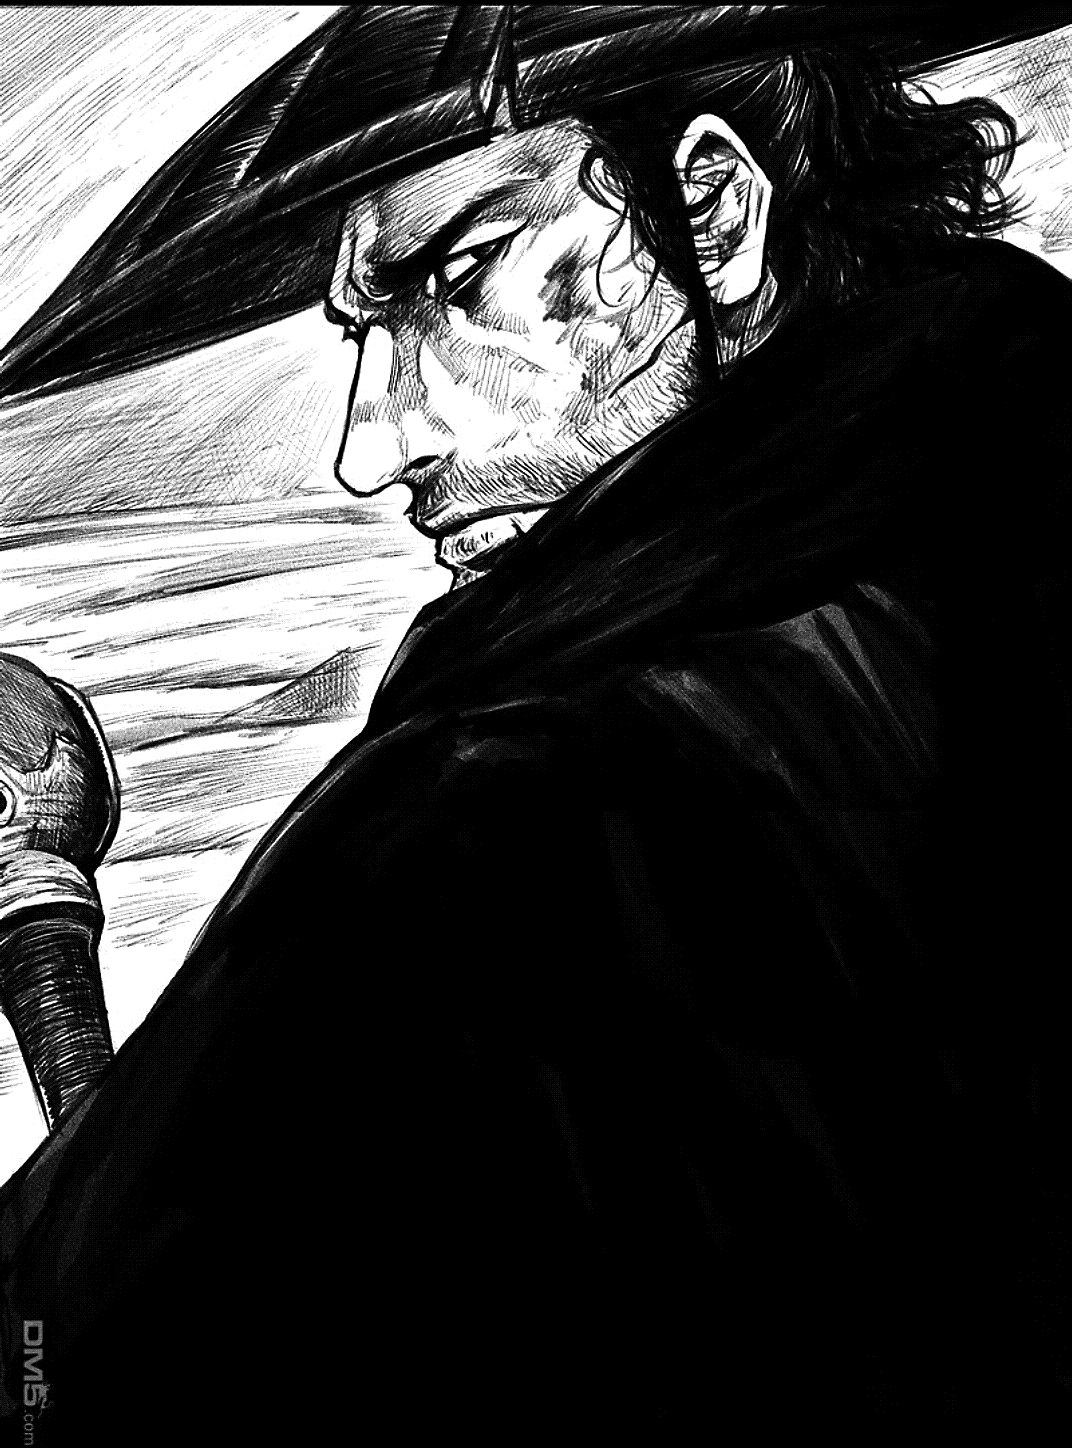
\includegraphics[width=0.30\textwidth]{xiantu.jpg}   %添加图片,文件名xiantu.jpg
    \caption{宋赵爽,给出了证明。\label{fig:xiantu}}     %图片下面的文字说明
\end{figure}

% 图二
\begin{figure}[!ht]\centering
    
\includegraphics[width=0.30\textwidth]{E:/Backgruond/1.jpg}
    \caption{自定义}
\end{figure}


\clearpage
% 第二节
\section{勾股定理的近代形式}



\begin{thm}[\small 勾股定理]    %开始定理环境
    \small 直角三角形斜边的平方等于两腰的平方和

    \small 可以用符号语言表述为:设直角三角形$ABC$,其中$\angle C=90 \degree$,则有
    %$$之间为数学表达式的书写地方,我们定义的degree是为了写度数符号
    \begin{equation}\label{eq:gougu}   %开始单行公式环境equation,并添加了数千gougu
        AB^2=BC^2+AC^2.
    \end{equation}
\end{thm}


\begin{thm}[\small 中值定理] 
    \small 中值定理
\end{thm}

\small 满足式 \eqref{eq:gougu} 的整数成为 \emph{勾股数}。第 \ref{sec:ancient} 节所说毕达哥拉斯学派得到的三元数就是勾股数。
%|eqref{eq:gougu}读入书签gougu;emph强调勾股数,ref读入书签ancient

\vspace{3mm}    %空一行
\begin{tabular}{|c|c|c|}\hline   %开始表格环境,{|c|c|c|}表示文字居中的三列,\hline表述画两条并排的水平线。必须用于行首或换行命令之后
    \small 直角边 $a$ & 直角边 $b$ & 斜边 $c$ \\\hline  %  &是数据分割符号
    3 & 4 & 5 \\\hline
    5 & 12 & 13 \\\hline
\end{tabular}
\small($a^2+b^2=c^2$)

\clearpage
% 参考文献
\addcontentsline{toc}{section}{参考文献} %用来添加文献的标准方式
\begin{thebibliography}{99}   %参考文献开始
    \bibitem{1} 失业健太郎.几何的有名定理.上海科学技术出版社,1986
    \bibitem{quanjing}全金.商高、赵爽与刘辉关于勾股定理的证明.数学传播,20(3),1998.
    \bibitem{Kline}克莱因.古今数学思想.上海科学技术出版社.2002.
\end{thebibliography}



% 附录
\begin{appendix}          %附录开始
\section{附录} %要写的附录
    \small 勾股定理又叫商高定理,国外也称百牛定理。    
\end{appendix}












\end{document}